% Preamble
% ---
\documentclass[paper=a4, fontsize=11pt]{scrartcl}

% Packages =========================================================================
% ---
\usepackage{geometry}
\geometry{
  a4paper,
  total={170mm,257mm},
  left=20mm,
  right=20mm,
  top=30mm,
  bottom=35mm,
}
\usepackage[utf8]{inputenc}   % UTF-8 support
\usepackage[french]{babel}
\usepackage{amsmath,amsfonts} % Advanced math typesetting
\usepackage{float}            % Place figures exactly where we want
\usepackage{graphicx}
\usepackage{listings}         % Source code formatting and highlighting
\usepackage{lastpage}         % Reference to last page
\usepackage[parfill]{parskip} % No indent at start of new line
\usepackage{color}
  \definecolor{codegreen}{rgb}{0,0.6,0}
  \definecolor{codegray}{rgb}{0.5,0.5,0.5}
  \definecolor{backcolour}{rgb}{0.95,0.95,0.92}
\usepackage{fancyhdr}         % Create headers and footers
	\pagestyle{fancy}

% Create horizontal rule command with 1 argument of height
\newcommand{\horrule}[1]{\rule{\linewidth}{#1}}

% Title page things ================================================================
\title{
  \normalfont \normalsize
  \textsc{HEIG-VD - Simulation et Optimisation} \\[10pt]
  \horrule{1pt} \\[0.4cm] % Thin top horizontal rule
  \huge Travail Pratique 2~:\\Méthode de Monte-Carlo \\
  \horrule{2pt} \\[0.4cm] % Thick bottom horizontal rule
}
\author{Luc \bsc{Wachter}}
\date{28 mai 2019}

% Header and footer things =========================================================
\renewcommand{\footrulewidth}{0.4pt}
\lhead{SIO - Travail pratique 2}
\rhead{Luc Wachter}
\lfoot{28.05.2019}
\cfoot{}
\rfoot{Page \thepage \ sur \pageref{LastPage}}

% Style for code listings ==========================================================
\lstdefinestyle{codestyle}{
    backgroundcolor=\color{backcolour},
    commentstyle=\color{codegreen},
    numberstyle=\tiny\color{codegray},
    basicstyle=\footnotesize,
    breakatwhitespace=true,
    breaklines=true,
    captionpos=b,
    keepspaces=true,
    numbers=left,
    numbersep=5pt,
    showspaces=false,
    showstringspaces=false,
    showtabs=false,
    tabsize=2
}
\lstset{style=codestyle}

% Document =========================================================================
% ---
\begin{document}

% Set language for code listings
\lstset{language=Java}

\maketitle

% Début Section ==================================================================
\section{Introduction}

Dans ce travail pratique, nous nous intéressons au calcul de la distance moyenne entre deux points du carré unité. Il s'agit donc de calculer l'espérance de la distance euclidienne séparant deux points indépendants et identiquement distribués dans le carré unité $[0;1] \times [0;1]$.

Si on note $P(x_1;y_1)$ et $Q(x_2;y_2)$ deux points du carré unité et $D$ la distance euclidienne qui les sépare, l'espérance de cette distance est
\begin{equation*}
  \text{E}(D) = \int _0^1\int _0^1\int _0^1\int _0^1\sqrt{\:\left(x_2-x_1\right)^2+\left(y_2-y_1\right)^2}dy_2dy_1dx_2dx_1.
\end{equation*}
C'est cette espérance que l'on veut calculer.

Pour ce faire, nous allons réaliser une simulation de Monte-Carlo afin de générer des estimateurs $\widehat{D}$ de $\text{E}(D)$ à partir d'échantillons de populations générées aléatoirement.

Ce document a pour but de documenter les choix faits durant la conception du programme, mais surtout de présenter les résultats obtenus, de les interpréter et de les discuter.

\newpage

% Début Section ==================================================================
\section{Correspondance des symboles}

Les symboles mathématiques proposés dans la donnée du travail ne sont bien sûr pas propices à une utilisation en Java. Le tableau \ref{table:correspondance} permet donc de faire le lien entre les symboles utilisés dans ce document et ceux utilisés dans le programme.

\begin{table}
  \centering
  \begin{tabular}{|l|l|}
    \hline
    Symbole mathématique & Symbole dans le code \\
    \hline
    $N_{init}$ & \texttt{initialNumberOfRuns} \\
    $N_{add}$ & \texttt{additionalNumberOfRuns} \\
    $N$ & \texttt{estimatedNumberOfRunsNeeded} \\
    $\Delta_{max}$ & \texttt{maxHalfWidth} \\
    $s$ & \texttt{standardDeviation} \\
    \hline
  \end{tabular}
  \caption{Correspondance des symboles}
  \label{table:correspondance}
\end{table}

% Début Section ==================================================================
\section{Choix du nombre d'expériences à effectuer}

Après avoir lancé la simulation pour exécuter $N_{init}$ expériences, il nous faut estimer le nombre d'expériences supplémentaires nécessaires pour arriver à un intervalle de confiance à 95\% dont la demi-largeur ne dépasse pas $\Delta_{max}$.

Ce nombre d'expériences $n$ peut être estimé en utilisant l'équation pour la largeur de l'intervalle de confiance~:
\begin{equation*}
  \Delta_{I_c} = 2\cdot z_{1-\frac{\alpha}{2}}\cdot \dfrac{s}{\sqrt{n}}
\end{equation*}

Adaptons cette équation pour notre cas pratique en remplaçant la largeur de l'intervalle de confiance $\Delta_{Ic}$ par la demi-largeur maximale $\Delta_{max}$ (valeur fixée par le code appelant). Ce changement nous permet de faire fi du facteur deux du côté droit de l'équation, puisque nous nous intéressons à la demi-largeur et non à la largeur complète.
\begin{equation*}
  \Delta_{max} = z_{1-\frac{\alpha}{2}}\cdot \dfrac{s}{\sqrt{n}}
\end{equation*}

Il nous suffit alors d'isoler $n$ pour déterminer la formule à utiliser dans notre programme.
\begin{align*}
  \Delta_{max} &= z_{1-\frac{\alpha}{2}}\cdot \dfrac{s}{\sqrt{n}} \\ \\
  \Rightarrow \ \sqrt{n} &= \dfrac{z_{1-\frac{\alpha}{2}}\cdot s}{\Delta_{I_c}} \\ \\
  \Rightarrow \ n &= \dfrac{z_{1-\frac{\alpha}{2}}^2\cdot s^2}{\Delta_{I_c}^2}
\end{align*}

En utilisant $1.959964$ comme quantile de la loi normale et avec l'estimateur $s$ de l'écart-type calculé empiriquement à l'aide de nos expériences initiales, il nous est donc possible d'estimer le nombre d'expériences nécessaires pour arriver à la précision voulue.

% Début Section ==================================================================
\section{Approche utilisée}

Afin d'obtenir les résultats qui seront discutés dans la section suivantes, 1500 simulations ont été lancées en séquence. Pour chacune d'entre elles, les paramètres suivants ont été fixés~:

$\Delta_{max} = 5\cdot 10^{-5}$,\hspace{20pt} $N_{init} = 10^6$,\hspace{20pt} $N_{add} = 10^5$

En outre, la séquence de nombres créés par le générateur pseudo-aléatoire dans le programme a été fixée à l'aide de la graine \texttt{20190528}.

Les valeurs ayant été enregistrées à la fin de chaque simulation sont le nombre d'observations effectuées, la valeur de l'estimateur calculé (la moyenne), l'écart-type, la variance et la demi-largeur de l'intervalle de confiance à 95\%.

% Début Section ==================================================================
\section{Résultats}

\subsection{Valeur exacte de l'espérance}

Afin d'analyser les résultats de la simulation, la valeur exacte de $\text{E}(D)$ nous est donnée.
\begin{align*}
  \text{E}(D) &= \int _0^1\int _0^1\int _0^1\int _0^1\sqrt{\:\left(x_2-x_1\right)^2+\left(y_2-y_1\right)^2}dy_2dy_1dx_2dx_1 \\ \\
  &= \dfrac{2 + \sqrt{2} + 5\ln{\sqrt{2} + 1}}{15} \\ \\
  &\approx 0,5214054
\end{align*}

Dans toutes les figures suivantes, cette valeur exacte sera mise en évidence par une droite de couleur verte.

\subsection{Distribution des estimateurs ponctuels $\widehat{D}$}

En observant l'histogramme de la figure \ref{fig:hist}, nous remarquons la forme caractéristique de la loi normale. L'apparition d'une telle distribution n'est pas surprenante, puisque nos $\widehat{D}$ sont calculés comme la moyenne des résultats d'expériences aléatoires indépendantes, et que le théorème central limite nous permet d'établir la convergence de la loi de ces expériences vers la loi normale.

Il y donc une tendance vers une distribution symétrique autour de la valeur exacte de l'espérance recherchée. On observe plus facilement, à l'aide de la boîte à moustache de la figure \ref{fig:boxplot} que la moyenne (représentée par un segment noir épais au centre de la boîte) se rapproche de la valeur exacte, et que les observations sont distribuées symétriquement et uniformément autour de cette valeur.

\begin{figure}[H]
  \centering
  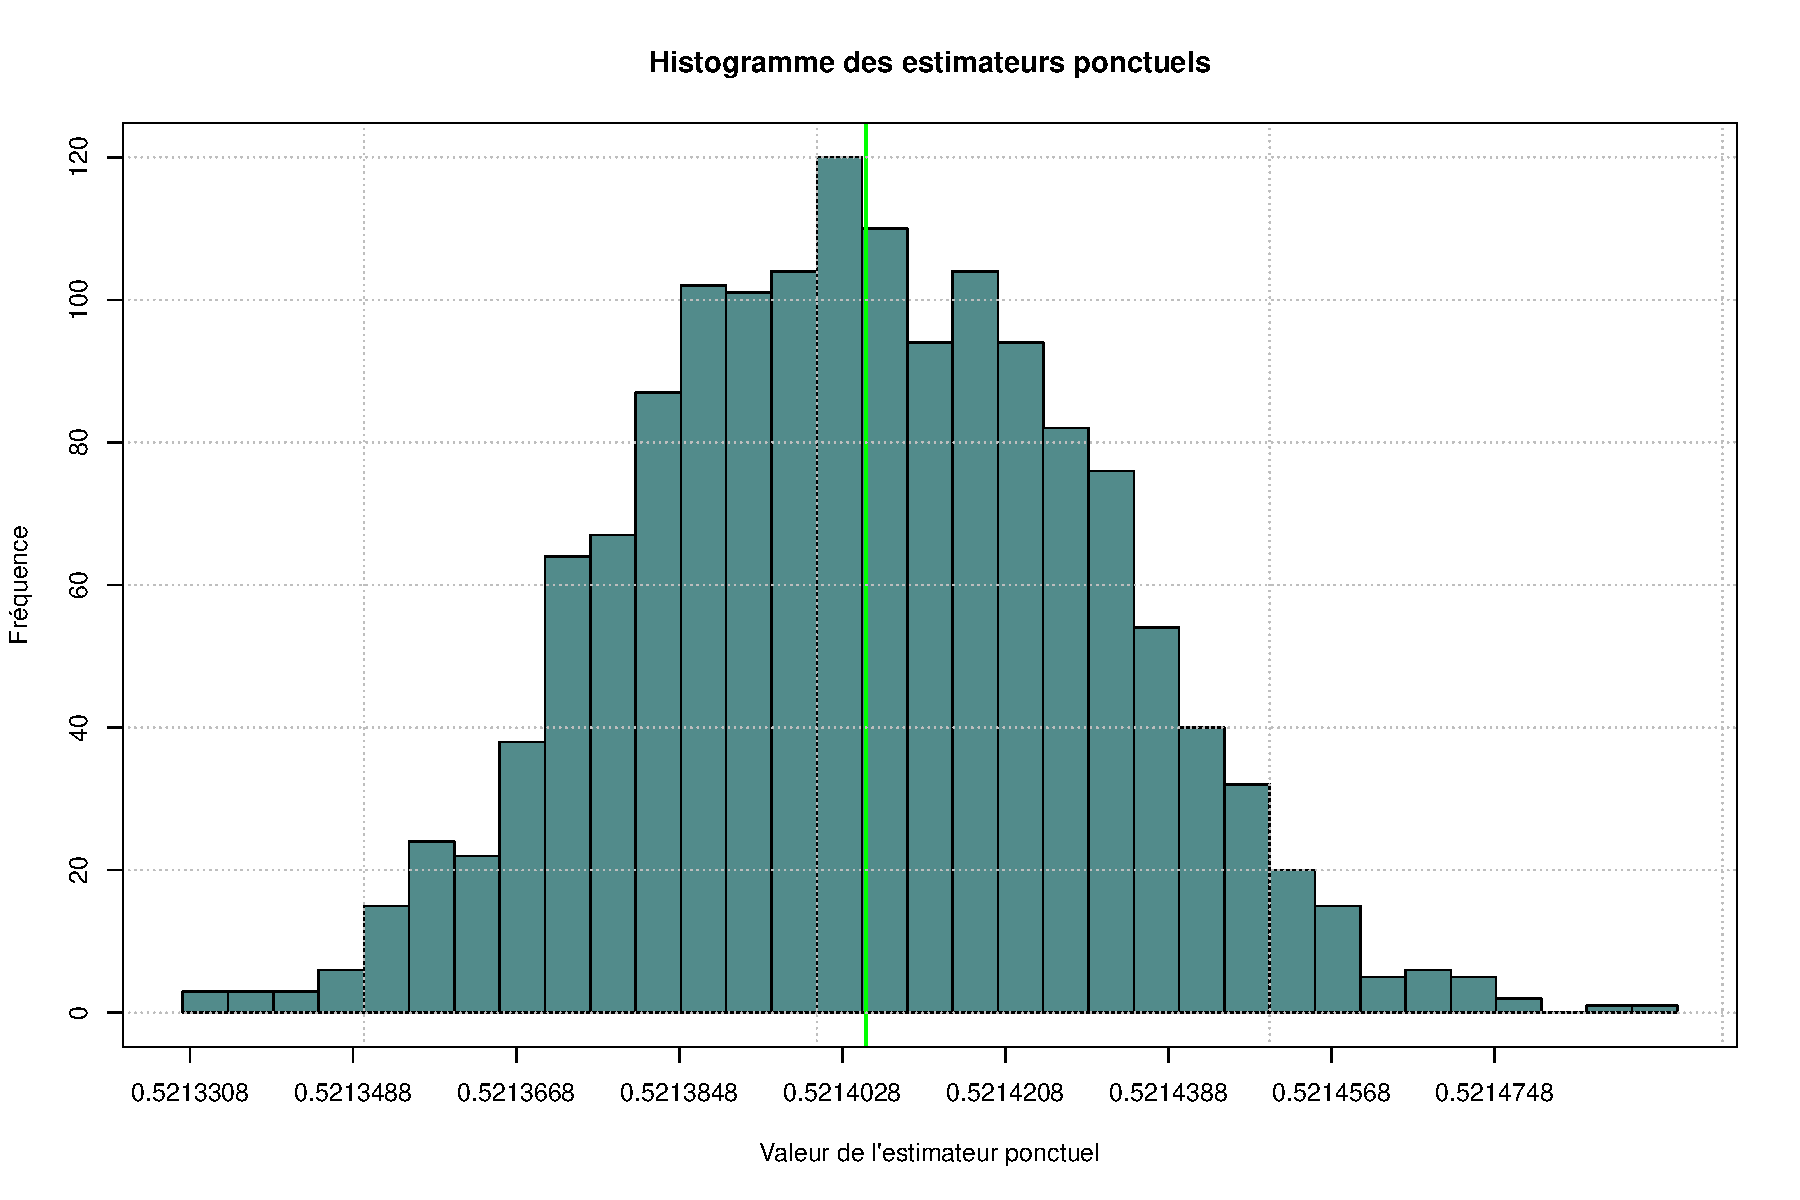
\includegraphics[scale=0.5]{../analysis/plots/EstimatorHistogram.pdf}
  \caption{Histogramme des estimateurs $\widehat{D}$}
  \label{fig:hist}
\end{figure}

\begin{figure}[H]
  \centering
  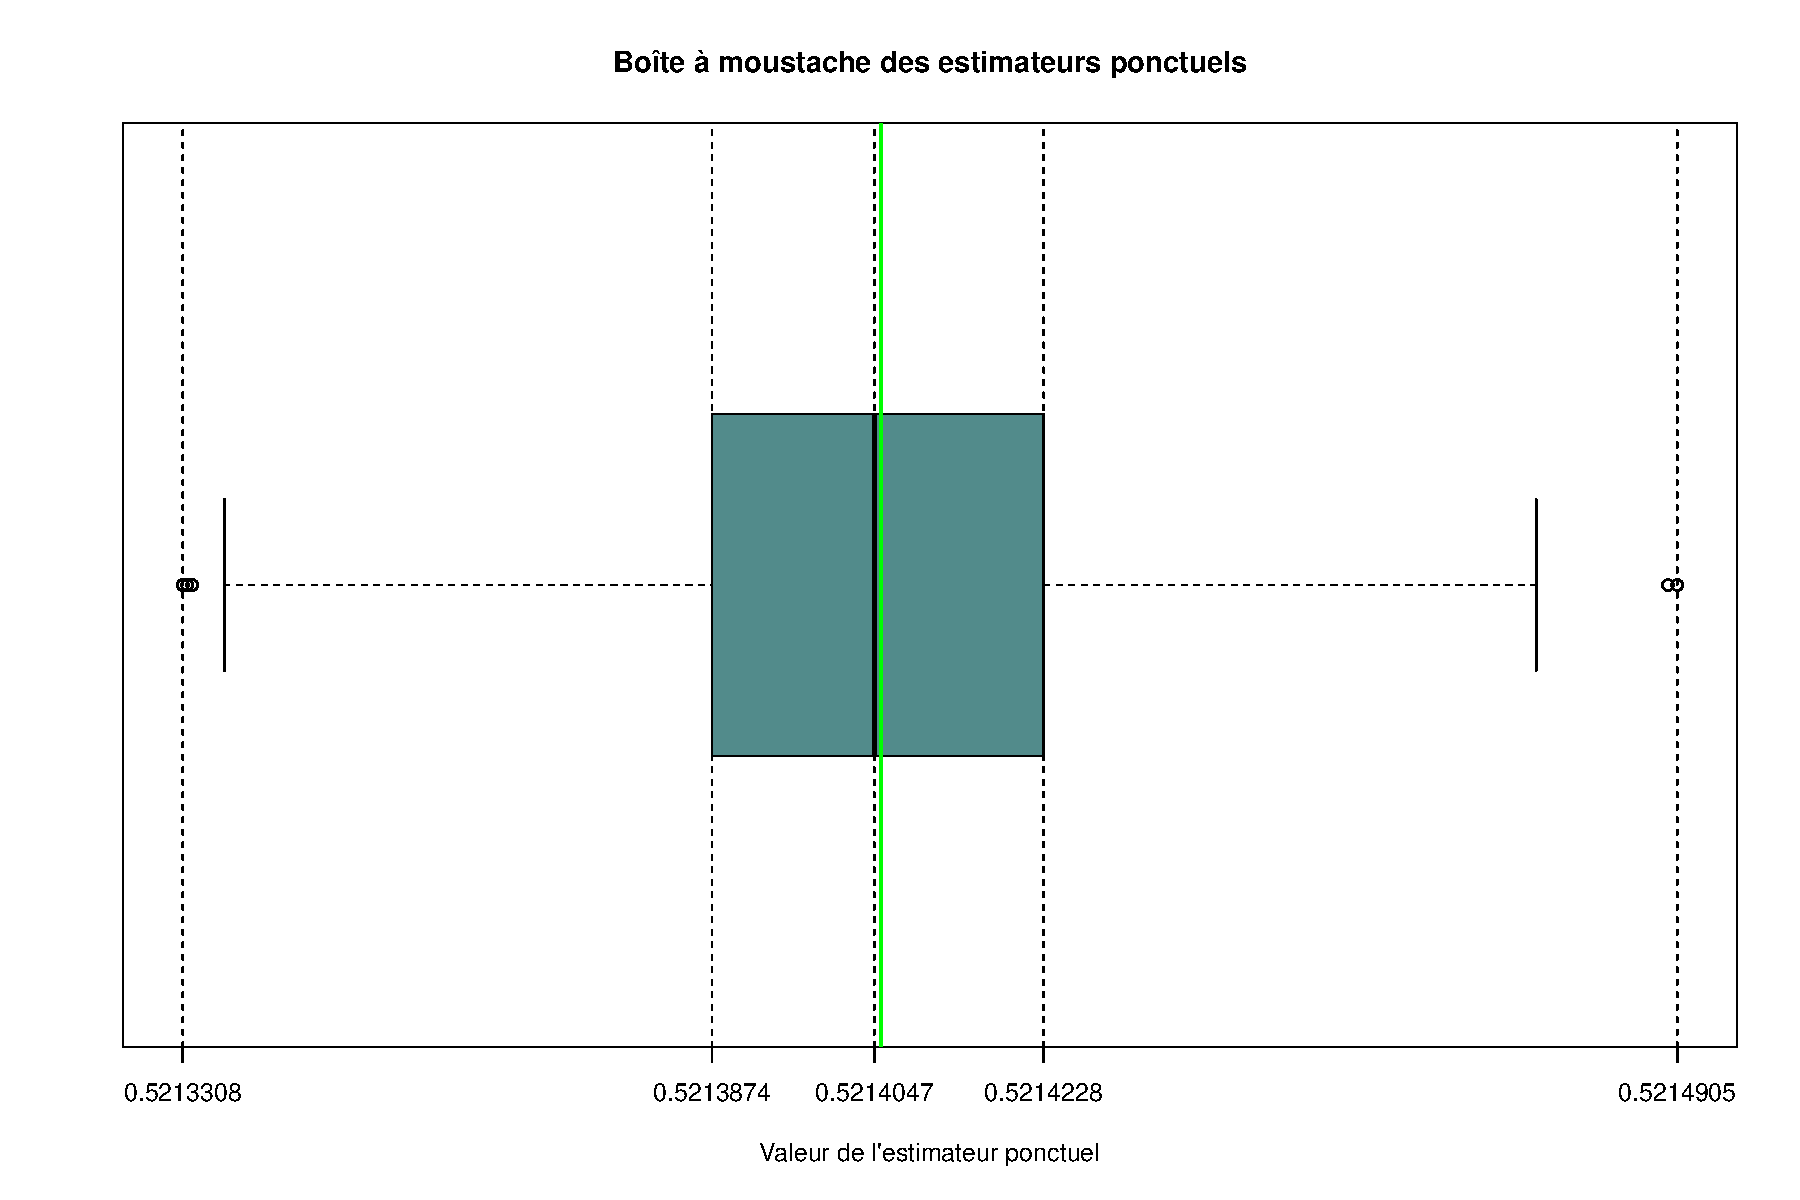
\includegraphics[scale=0.5]{../analysis/plots/BoxPlot.pdf}
  \caption{Boîte à moustache des estimateurs $\widehat{D}$}
  \label{fig:boxplot}
\end{figure}

\subsection{Couverture empirique des intervalles de confiance}

À l'aide du graphique des intervalles de confiance de la figure \ref{fig:CIPlot}, nous pouvons visualiser les intervalles de confiance des 100 premières simulations effectuées. Sur cette figure, les points représentent la valeur de l'estimateur $\widehat{D}$, tandis que les barres montrent l'I.C. pour chaque estimateur. Les éléments en rouge sont ceux dont l'I.C. ne contient pas la valeur exacte de l'espérance recherchée.

On observe une distribution cohérente par rapport à l'histogramme de la figure \ref{fig:hist}. On peut également remarquer que 3 estimateurs sont si éloignés que leur I.C. ne contient pas la valeur exacte. Cela signifie que le seuil de confiance empirique de cet échantillon des données s'élève à 97\%.

\begin{figure}[H]
  \centering
  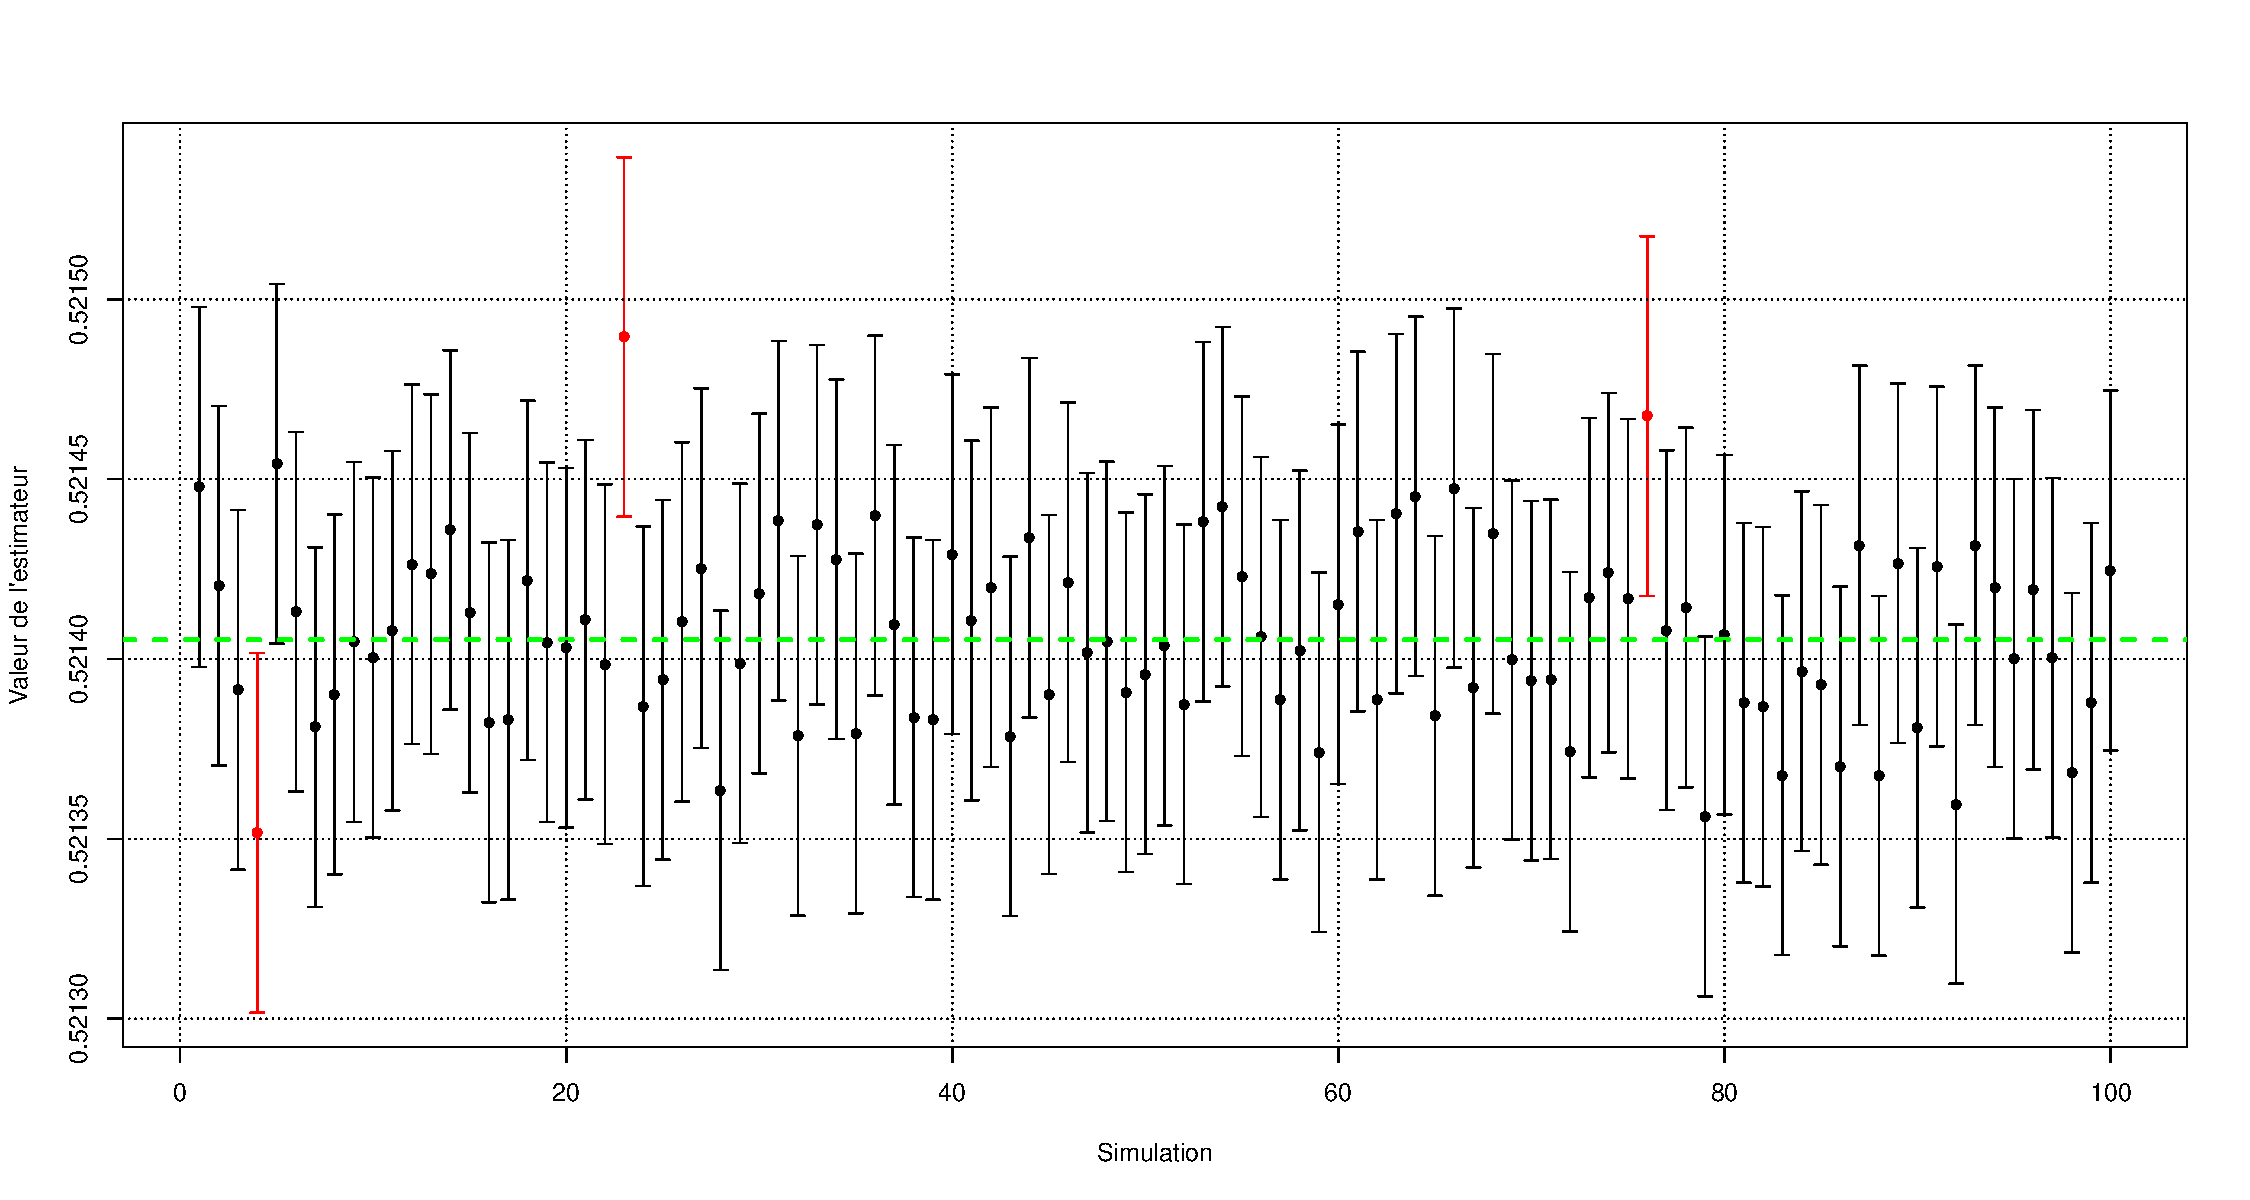
\includegraphics[scale=0.46]{../analysis/plots/CIplot.pdf}
  \caption{100 intervalles de confiance au seuil de 95\%}
  \label{fig:CIPlot}
\end{figure}

Augmentons maintenant la portée de notre analyse en regardant la totalité des simulations, à l'aide du nuage de points de la figure \ref{fig:PointsCloud}. Ici, les deux droites rouges valent respectivement $\text{E}(D) \pm \Delta_{max}$. On compte alors 62 estimateurs en dehors de cet intervalle (4.133\% des estimateurs générés), ce qui donne un seuil de confiance empirique de 95.867\%.

\begin{figure}[H]
  \centering
  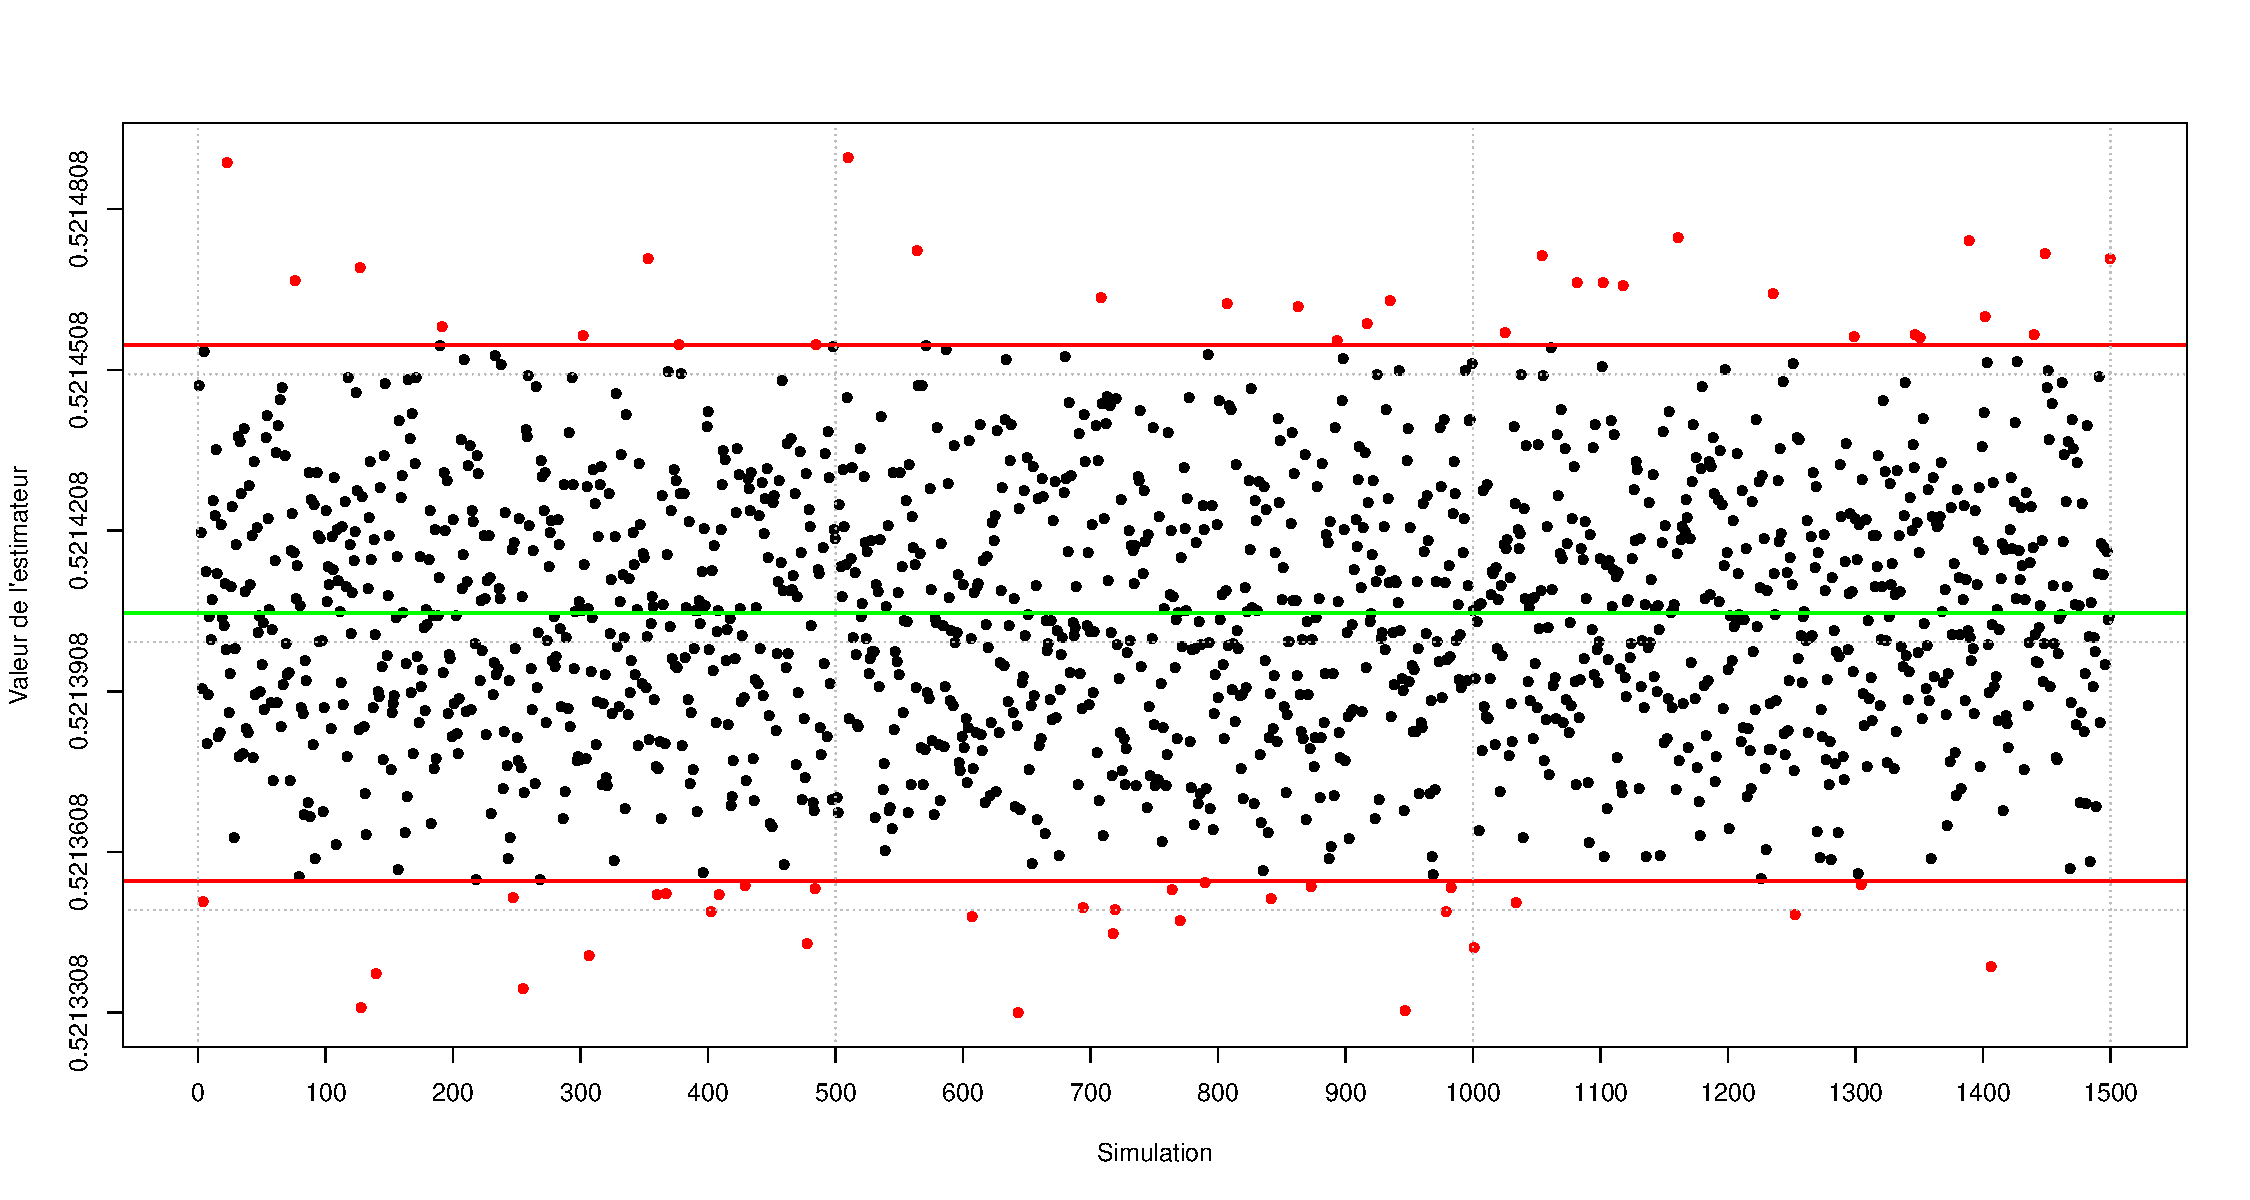
\includegraphics[scale=0.46]{../analysis/plots/PointsCloud.pdf}
  \caption{Nuage de points}
  \label{fig:PointsCloud}
\end{figure}

% Début Section ==================================================================
\section{Conclusion}

Au fur et à mesure de ce travail pratique, nous nous sommes efforcés d'estimer la valeur de $\text{E}(D)$ empiriquement. Il est clair cependant, que ce n'était pas le vrai but de ce travail. En effet, il est plus important de nous sensibiliser à la juste utilisation des méthodes approchées.

Grâce à ce travail, nous avons pu remarquer empiriquement qu'une simulation ne vaut pas grand chose si l'on ne quantifie pas l'erreur à l'aide de l'intervalle de confiance. En outre, même avec l'assurance d'atteindre un intervalle de confiance précis, il est toujours possible de se retrouver bien plus éloigné de la valeur exacte qu'on le voudrait en pratique. Il faut donc toujours avoir un regard critique sur les résultats des méthodes approchées.

Dans ce travail, cependant, nos observations empiriques nous ont permis de confirmer les intuitions acquises durant le cours. Nous avons vu qu'il est difficile de réduire la largeur de l'intervalle de confiance et nous avons confirmé par des observations les valeurs des intervalles de confiance, et la distribution des estimateurs.

\end{document}
